\documentclass[aspectratio=169,11pt]{beamer}
\usepackage[utf8]{inputenc}
\usepackage[T1]{fontenc}
\usepackage[brazil]{babel}
\usepackage{graphicx}
\usepackage{booktabs}
\usepackage{helvet}
\renewcommand{\familydefault}{\sfdefault}

% ---------- paleta clean ----------
\definecolor{primary}{HTML}{2C3E50}   % azul-ardósia (títulos/estrutura)
\definecolor{accent}{HTML}{18BC9C}    % verde-água (destaques)
\definecolor{darktext}{HTML}{22303C}
\definecolor{softgray}{HTML}{8A97A0}

\usetheme{default}
\setbeamertemplate{navigation symbols}{}
\setbeamercolor{normal text}{fg=darktext}
\setbeamercolor{structure}{fg=primary}
\setbeamercolor{frametitle}{fg=primary}
\setbeamerfont{frametitle}{series=\bfseries,size=\Large}
\setbeamerfont{title}{series=\bfseries}
\setbeamercolor{itemize item}{fg=accent}
\setbeamercolor{itemize subitem}{fg=accent}
\setbeamertemplate{itemize item}{\small\raisebox{0.12ex}{\textbf{--}}}
\setbeamertemplate{itemize subitem}{\scriptsize\raisebox{0.15ex}{$\bullet$}}

% título de frame limpo com régua de destaque
\setbeamertemplate{frametitle}{%
  \vspace{0.7em}\hspace{0.2em}\usebeamerfont{frametitle}\usebeamercolor[fg]{frametitle}\insertframetitle\par
  \vspace{0.15em}{\color{accent}\rule{\dimexpr\textwidth\relax}{1.6pt}}\par\vspace{-0.2em}%
}
% rodapé minimalista (número da página)
\setbeamertemplate{footline}{%
  \hspace*{\fill}{\color{softgray}\scriptsize\insertframenumber\,/\,\inserttotalframenumber}\hspace{1.2em}\vspace{0.7em}%
}

\newcommand{\hi}[1]{{\color{accent}\textbf{#1}}}   % destaque em verde-água
\newcommand{\pr}[1]{{\color{primary}\textbf{#1}}}  % destaque em azul

\begin{document}

% ===================== SLIDE 1 -- INTRO / CAPA =====================
\begin{frame}[plain]
\vspace{0.4em}
{\color{primary}\bfseries\Large Cálculo Paralelo do Conjunto de Mandelbrot}\\[2pt]
{\color{accent}\large\bfseries Versão Híbrida MPI + OpenMP}\\[3pt]
{\color{softgray}\footnotesize Bernardo Luiz Padilha Zamin \;\textbullet\; João Pedro Sostruznik Sotero da Cunha \;\textbullet\; Prog.\ Paralela --- T4 --- PUCRS}\\[3pt]
{\color{accent}\rule{\textwidth}{1.6pt}}
\vspace{0.7em}

\begin{columns}[c]
\begin{column}{0.58\textwidth}
\small
\textbf{Dois níveis de paralelismo} (imagem 7680$\times$4320):
\begin{itemize}\setlength{\itemsep}{4pt}
  \item \pr{Entre nós (MPI)} --- \emph{Coordenador/Trabalhador}: distribui blocos de linhas sob demanda; \hi{1 processo pesado por nó}.
  \item \pr{Dentro do nó (OpenMP)} --- \emph{workpool sem mestre}: todas as threads pegam a próxima linha de uma \hi{estrutura de dados} (\texttt{atomic capture}).
\end{itemize}
\smallskip
Carga \textbf{irregular} $\Rightarrow$ \hi{balanceamento dinâmico}. Rodado em \hi{4 nós} do Atlantica.
\end{column}
\begin{column}{0.42\textwidth}
\centering
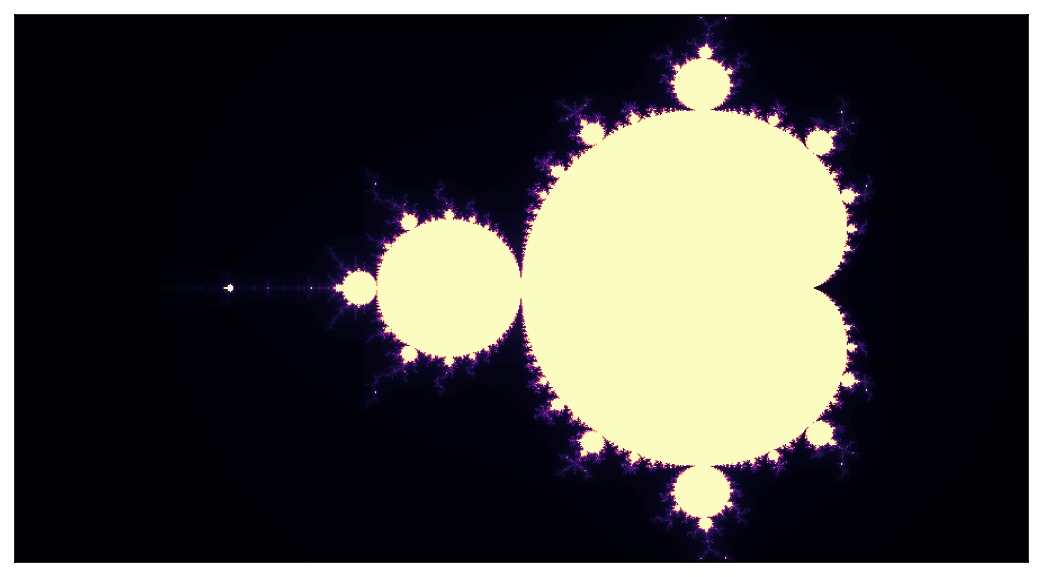
\includegraphics[width=\linewidth]{fig_mandel.png}\\[2pt]
{\color{softgray}\scriptsize Cor $=$ nº de iterações até escapar.}
\end{column}
\end{columns}
\end{frame}

% ===================== SLIDE 2 -- GRAFICOS E TABELAS =====================
\begin{frame}{Resultados}
\begin{columns}[c]
\begin{column}{0.60\textwidth}
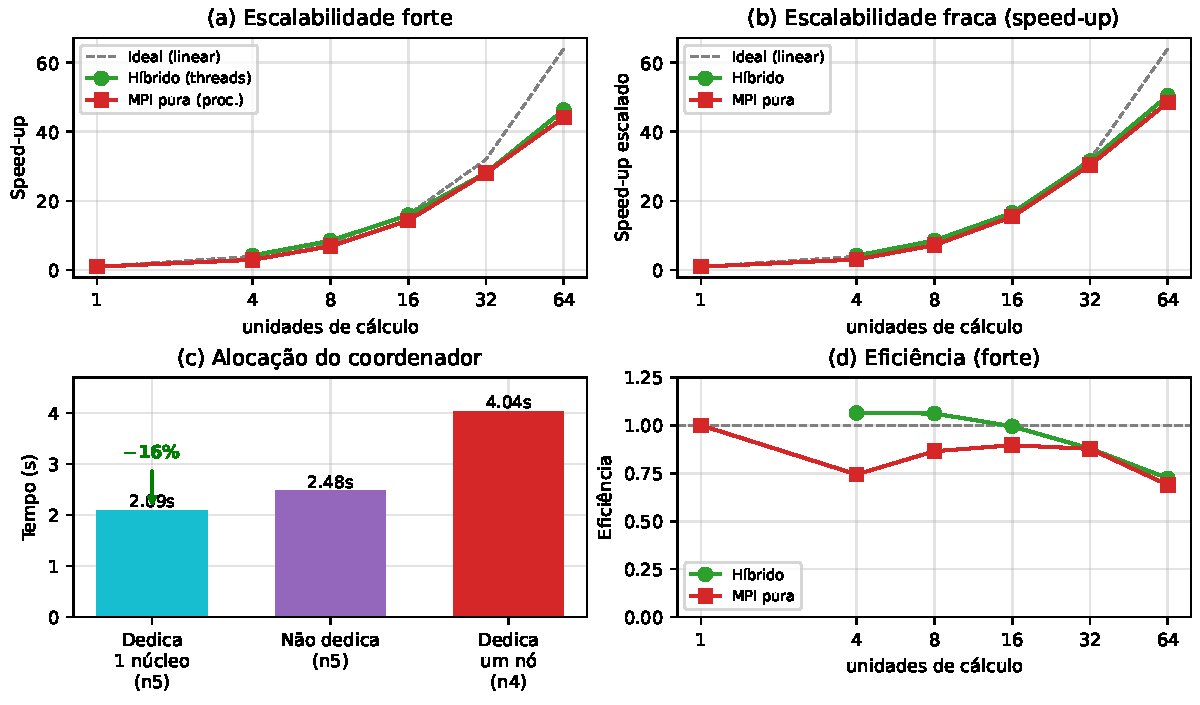
\includegraphics[width=\linewidth]{graficos.pdf}
\end{column}
\begin{column}{0.39\textwidth}
\scriptsize
{\color{primary}\textbf{Escalabilidade forte}} \, (speed-up $S$ / efic.\ $E$)\\[2pt]
\setlength{\arrayrulewidth}{0.3pt}
\begin{tabular}{r rr rr}
\toprule
& \multicolumn{2}{c}{\color{primary}Híbrido} & \multicolumn{2}{c}{\color{primary}MPI pura} \\
\cmidrule(lr){2-3}\cmidrule(lr){4-5}
un. & $S$ & $E$ & $S$ & $E$ \\ \midrule
1  & ---  & ---  & 1,00 & 1,00 \\
4  & 4,26 & 1,06 & 2,97 & 0,74 \\
8  & 8,49 & 1,06 & 6,92 & 0,86 \\
16 & 15,9 & 0,99 & 14,3 & 0,90 \\
32 & 28,1 & 0,88 & 28,1 & 0,88 \\
64 & \hi{46,3} & 0,72 & \hi{44,1} & 0,69 \\ \bottomrule
\end{tabular}

\vspace{5pt}
\begin{minipage}[t]{0.44\textwidth}
{\color{primary}\textbf{Fraca}} (speed-up)\\[2pt]
\begin{tabular}{r rr}
\toprule
un. & Híb. & MPI \\ \midrule
4  & 4,2  & 3,1 \\
16 & 16,6 & 15,5 \\
32 & 31,5 & 30,3 \\
64 & \hi{50,4} & \hi{48,5} \\ \bottomrule
\end{tabular}
\end{minipage}\hfill
\begin{minipage}[t]{0.52\textwidth}
{\color{primary}\textbf{Coordenador}} (4 nós)\\[2pt]
\begin{tabular}{l r}
\toprule
Alocação & Tempo \\ \midrule
Dedica 1 núcleo & \hi{2,09s} \\
Não dedica      & 2,48s \\
Dedica um nó    & 4,04s \\ \bottomrule
\end{tabular}
\end{minipage}

\vspace{4pt}
{\color{softgray}\tiny un.\ de cálculo $=$ núcleos (híbrido) / processos (MPI pura).}
\end{column}
\end{columns}
\end{frame}

% ===================== SLIDE 3 -- CONCLUSAO =====================
\begin{frame}{Conclusões}
\begin{itemize}
  \item Cumprimos o modelo: \pr{MPI Coordenador/Trabalhador} (1 processo pesado/nó) $+$ \pr{workpool OpenMP sem mestre} (controle por estrutura de dados, 2 threads/núcleo com HT).
  \medskip
  \item \textbf{Boa escalabilidade}: speed-up de \hi{46$\times$} (forte) e \hi{50$\times$} (fraca) em 64 unidades --- escalabilidade fraca quase ideal.
  \medskip
  \item A queda de eficiência em 64 unidades é o \hi{limite do Hyper-Threading} (2 fluxos/núcleo), não do algoritmo; no início há \emph{superlinearidade} por melhor uso de \textbf{cache}.
  \medskip
  \item \textbf{Alocação do coordenador}: vale dedicar \hi{1 núcleo} ($-16\%$, evita oversubscrição), mas \hi{nunca um nó} inteiro ($+63\%$).
  \medskip
  \item \pr{Híbrido $\times$ MPI pura}: desempenho \textbf{praticamente igual}, mas o híbrido usa \hi{muito menos ranks} MPI (5 vs 64) --- menos memória e mensagens, vantagem que cresce com a escala.
\end{itemize}
\end{frame}

\end{document}
